%
% strahlensatz.tex
%
% (c) 2018 Prof Dr Andreas Müller, Hochschule Rapperswil
%
\documentclass[tikz,12pt]{standalone}
\usepackage{times}
\usepackage{amsmath}
\usepackage{txfonts}
\usepackage[utf8]{inputenc}
\usepackage{graphics}
\usepackage{color}
\usepackage{pifont}
\usetikzlibrary{arrows,intersections,math,calc}
\begin{document}

\def\punkt#1{
        \fill[color=white] #1 circle[radius=0.08];
        \draw #1 circle[radius=0.08];
}

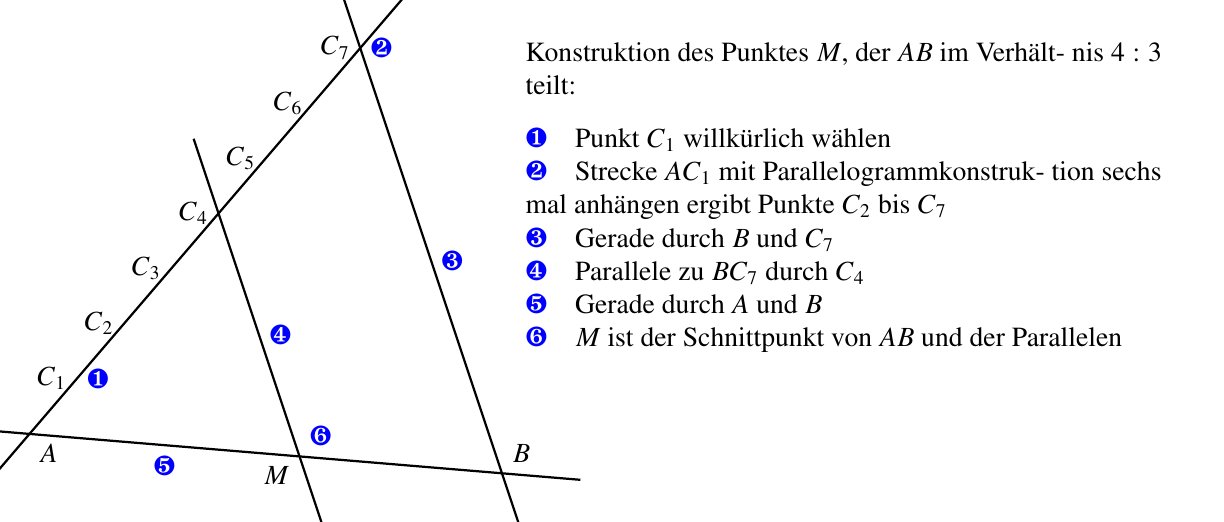
\begin{tikzpicture}[>=latex,thick]

\coordinate (A) at (0,0);
\coordinate (B) at (6,-0.5);
\coordinate (C) at (0.6,0.7);
\coordinate (C1) at ($1*(C)$);
\coordinate (C2) at ($2*(C)$);
\coordinate (C3) at ($3*(C)$);
\coordinate (C4) at ($4*(C)$);
\coordinate (C5) at ($5*(C)$);
\coordinate (C6) at ($6*(C)$);
\coordinate (C7) at ($7*(C)$);
\coordinate (M) at ($4/7*(B)$);

\draw[shorten >= -1cm,shorten <= -1cm] (A) to (B);

\draw[shorten >= -1cm,shorten <= -1cm] (A) to (C7);

\draw[shorten >= -1cm,shorten <= -1cm] (C7) to (B);
\draw[shorten >= -1cm,shorten <= -1cm] (M) to (C4);

\punkt{(C1)} \node at (C1) [left] {$C_1$};
\punkt{(C2)} \node at (C2) [left] {$C_2$};
\punkt{(C3)} \node at (C3) [left] {$C_3$};
\punkt{(C4)} \node at (C4) [left] {$C_4$};
\punkt{(C5)} \node at (C5) [left] {$C_5$};
\punkt{(C6)} \node at (C6) [left] {$C_6$};
\punkt{(C7)} \node at (C7) [left] {$C_7$};

\punkt{(A)} \node at (A) [below right] {$A$};
\punkt{(B)} \node at (B) [above right] {$B$};
\punkt{(M)} \node at (M) [below left] {$M$};

\node[color=blue] at (C1) [right] {\ding{182}};
\node[color=blue] at (C7) [right] {\ding{183}};
\node[color=blue] at ($0.5*(C7)+0.5*(B)$) [right] {\ding{184}};
\node[color=blue] at ($0.286*(C7)+0.286*(B)$) [right] {\ding{185}};
\node[color=blue] at ($0.286*(B)$) [below] {\ding{186}};
\node[color=blue] at (M) [above right] {\ding{187}};

\node at (10.5,3) {%
\begin{minipage}{8.4cm}
\parindent0pt
\raggedright
Konstruktion des Punktes $M$, der $AB$ im Verhält- nis $4:3$ teilt:
\\[7pt]
{\color{blue}\ding{182}}\quad%
Punkt $C_1$ willkürlich wählen\\
{\color{blue}\ding{183}}\quad%
Strecke $AC_1$ mit Parallelogrammkonstruk- tion sechs mal anhängen ergibt
Punkte $C_2$ bis $C_7$\\
{\color{blue}\ding{184}}\quad%
Gerade durch $B$ und $C_7$\\
{\color{blue}\ding{185}}\quad%
Parallele zu $BC_7$ durch $C_4$\\
{\color{blue}\ding{186}}\quad%
Gerade durch $A$ und $B$\\
{\color{blue}\ding{187}}\quad%
$M$ ist der Schnittpunkt von $AB$ und der Parallelen\\
\end{minipage}};

\end{tikzpicture}

\end{document}

